\chapter{Probability Distributions}\label{c2}
\section{Multinomial variables}\label{c2s1}
A multinomial variable can take one out of $K$ possible values. One can express it as a variable
with a range restricted to $K$ integers, typically $1$ to $K$. Alternatively, we can express it as 
a boolean  $K$ vector where exactly one component is $1$ and the rest are $0$. We choose the latter 
alternative. We use the notation customary in linear algebra to denote the boolean vector with just 
the $k$-th component $1$ and the remaining ones zero by $e_k$.

Let a multinomial variable $X$ take a value $k$ with probability $\mu_k$. Then 
\[
\sum_{k=1}^K \mu_k = 1
\]
and 
\begin{equation}\label{c2s1e1}
p(X = e_k|\mu) = \prod_{k=1}^K \mu_k^{x_k},
\end{equation}
where $x_k$ is the $k$th component of the boolean $K$-vector representing the state
$X = k$. Every component of the vector contributes a $1$ to the product except the
one with $x_k = 1$, which contributes $\mu_k$. Therefore,
\[
p(X = e_k|\mu) = \mu_k
\]
and hence
\begin{equation}\label{c2s1e2}
\sum_{k=1}^K`p(X = e_k|\mu) = 1.
\end{equation}

The expectation of a multinomial random variable is
\begin{equation}\label{c2s1e3}
\ev(X|\mu) = \sum_{k=1}^K e_kp(X = e_k|\mu) = (\mu_1, \ldots, \mu_K) = \mu.
\end{equation}
A dataset $\mathcal{D}$ of $N$ i.i.d. multinomial random variables has a prior probability
\[
p(\mathcal{D}|\mu) = \prod_{n=1}^Np(X_n = e_k|\mu) = \prod_{n=1}^N\prod_{k=1}^K \mu_k^{(x_n)_k}.
\]
In this equation, the data set has vectors ${x_1, \ldots, x_N}$, all in $\{0, 1\}^K$ and whose
$k$-th component is denoted by $(x_n)_k$. We can simplify the previous equation as
\[
p(\mathcal{D}|\mu) = \prod_{k=1}^K \mu_k^{\sum_{n=1}^N (x_n)_k}.
\]
The sum 
\[
\sum_{n=1}^N (x_n)_k
\]
is the number of $x_n$ whose $k$th component is $1$, that is the number of $x_n = e_k$. Let
us call this number $m_k$, Then
\begin{equation}\label{c2s1e4}
p(\mathcal{D}|\mu) = \prod_{k=1}^K \mu_k^{m_k}.
\end{equation}
It is clear that 
\begin{equation}\label{c2s1e5}
\sum_{k=1}^K m_k = N.
\end{equation}

We could have arrived at equation \eqref{c2s1e4} with a much simpler analysis. If the probability
that a multinomial random variable takes a value $k$ is $\mu_k$ and if a data set of $N$ such
variables has $m_k$ variables taking the value $k$ then
\[
p(\mathcal{D}|\mu) = \prod_{k=1}^K \mu_k^{m_k}.
\]
We took the longer route only to demonstrate how to work with boolean $K$-vectors.

In order to find the maximum-likelihood estimate of the $\mu$, we maximize the logarithm of
equation \eqref{c2s1e4} subject to the constraint $\sum_{k=1}^K \mu_k = 1$. If $\lambda$ is
the Lagrange's undermined multiplier then we consider the function
\[
f(\mu_k) = \sum_{k=1}^Lm_k\ln{\mu_k} + \lambda\left(\sum_{k=1}^K \mu_k - 1\right)
\]
and its derivative
\[
\frac{df}{d\mu_k} = \frac{m_k}{\mu_k} + \lambda.
\]
The maximum likelihood estimate of $\mu$ is thus,
\begin{equation}\label{c2s1e6}
\mu_{ML} = -\frac{1}{\lambda}(m_1, \ldots, m_K).
\end{equation}
The multiplier $\lambda$ can be found by substituting the previous equation in the equation
of constraint. Thus,
\[
\sum_{k=1}^K \mu_k = -\sum_{k=1}^K \frac{m_k}{\lambda} = -\frac{1}{\lambda}\sum_{k=1}^K m_k = 1.
\]
From equation \eqref{c2s1e5} we have
\[
\lambda = -\frac{1}{N}.
\]
Therefore the maximum-likelihood estimate of \eqref{c2s1e6} becomes
\begin{equation}\label{c2s1e7}
\mu_{ML} = \left(\frac{m_1}{N}, \ldots, \frac{m_k}{N}\right).
\end{equation}

\section{Problems}\label{c2p}
\begin{enumerate}
\item The Bernoulli distribution is defined as $\mathrm{Bern}(x|\mu) = \mu^x(1 - \mu)^x$. The 
random variable can take only two values, $0$ and $1$. Clearly, $p(X=0|\mu) = 1 - \mu$ and 
$p(X=1|\mu) = \mu$ so that
\[
\sum_x p(x|\mu) = 1.
\]
The expectation value of $X$ is
\[
\ev(X) = \sum_x xp(x|\mu) = 0\cdot(1 - \mu) + 1\cdot\mu = \mu.
\]
The variance of $X$ is
\[
\var(X) = \sum_x \ev(x - \mu)^2 = (0 - \mu)^2(1 - \mu) + (1 - \mu)^2\mu = \mu(1 - \mu).
\]

\item Given that
\[
p(x|\mu) = \left(\frac{1-\mu}{2}\right)^{(1-x)/2}\left(\frac{1+\mu}{2}\right)^{(1+x)/2},
\]
where $x \in {-1, 1}$ and $\mu \in [0, 1]$. Then $p(X=-1|\mu) = (1 - \mu)/2$ and $p(X=1|\mu)
= (1 + \mu)/2$ so that 
\[
\sum_x p(x|\mu) = 1.
\]
The expectation value of $X$ is
\[
\ev(X) = \sum_x xp(x|\mu) = -1\cdot\frac{1 - \mu}{2} + 1\cdot\frac{1 + \mu}{2} = \mu.
\]
We also find
\[
\ev(X^2) = \frac{1 - \mu}{2} + \frac{1 + \mu}{2} = 1
\]
so that $\var(X) = 1 - \mu^2$. We verify the variance using the other form,
\[
\var(X) = (-1 - \mu)^2\frac{1 - \mu}{2} + (1 - \mu)^2\frac{1 + \mu}{2} = 1 - \mu^2.
\]

\item We can show that the binomial distribution is normalized by evaluating the sum,
\[
\sum_{m=0}^N\binom{N}{m}\mu^m(1 - \mu)^{N-m} = (\mu + 1 - \mu)^N = 1.
\]
We used the binomial theorem to get the first equality.

\item Consider the expression,
\[
\sum_{k=0}^N \binom{N}{k}\mu^k(1 - \mu)^{N-k} = 0.
\]
Differentiate it with respect to $\mu$. Recall that $\mu \in [0, 1]$ so that the differentiation 
is well defined.
\[
\sum_{k=0}^N\binom{N}{k}k\mu^{k-1}(1 - \mu)^{N-k} - \sum_{k=0}^N\binom{N}{k}(N-k)\mu^k(1 - \mu)^{N-k-1} = 0.
\]
Multiply throughout by $\mu$ to get
\[
\sum_{k=0}^N\binom{N}{k}\mu^k(1 - \mu)^{N-k} = \mu N\sum_{k=0}^{N-1}\binom{N-1}{k}\mu^k(1 - \mu)^{N-k-1}.
\]
The left hand side is $\bar{X}$ while the right hand side is $\mu N$.

\item Consider the product
\[
\Gamma(a)\Gamma(b) = \int_0^\infty e^{-x}x^{a-1}dx\int_0^\infty e^{-y}y^{b-1}dy = \iint_{Q_1}e^{-x-y} x^{a-1}y^{b-1}dxdy,
\]
where $Q_1$ is the first quadrant. To evaluate this integral, introduce the variables $x = zt$
and $y = z(1 - t)$ or $z = x + y$ and $t = x/(x + y)$. The variable $z$ ranges from $0$ to 
$\infty$ while $t$ goes from $0$ to $1$. The jacobian of the transformation is
\[
\frac{\partial(x, y)}{\partial(z, t)} = \begin{vmatrix} x_z & x_t \\ y_z & y_t \end{vmatrix}
= \begin{vmatrix} t & z \\ 1 - t & -z \end{vmatrix} = -z.
\]
Therefore, 
\[
\Gamma(a)\Gamma(b) = \int_0^\infty\int_0^1 e^{z} z^{a-1}t^{a-1}z^{b-1}(-t)^{b-1}\abs*{\frac{\partial(x, y}{\partial(z, t)}}dzdt.
\]
The $z$ and the $t$ integrals factor out, so that
\[
\Gamma(a)\Gamma(b) = \int_0^\infty e^z z^{a+b-1}dz\int_0^1 t^{a-1}(1 - t)^{b- 1}dt = \Gamma(a+b)B(a, b).
\]

\item The mean of beta distribution is
\begin{eqnarray*}
\ev(X) &=& \frac{\Gamma(a+b)}{\Gamma(a)\Gamma(b)}\int_0^1 x B(x|a, b)dx \\
 &=& \frac{\Gamma(a+b)}{\Gamma(a)\Gamma(b)}\int_0^1x^a(1 - x)^{b-1}dx \\
 &=& \frac{\Gamma(a+b)}{\Gamma(a)\Gamma(b)}\frac{\Gamma(a+1)\Gamma(b)}{\Gamma(a+b+1)} \\
 &=& \frac{a}{a+b}.
\end{eqnarray*}
Likewise,
\begin{eqnarray*}
\ev(X^2) &=& \frac{\Gamma(a+b)}{\Gamma(a)\Gamma(b)}\int_0^1 x^2 B(x|a, b)dx \\
 &=& \frac{\Gamma(a+b)}{\Gamma(a)\Gamma(b)}\int_0^1x^{a+2}(1 - x)^{b-1}dx \\
 &=& \frac{\Gamma(a+b)}{\Gamma(a)\Gamma(b)}\frac{\Gamma(a+2)\Gamma(b)}{\Gamma(a+b+2)} \\
 &=& \frac{a(a+1)}{(a+b)(a+b+1)}.
\end{eqnarray*}
Therefore,
\[
\var{X} = \frac{a(a+1)}{(a+b)(a+b+1)} - \frac{a^2}{(a+b)^2} = \frac{ab}{(a+b)^2(a+b+1)}.
\]

The mode of the distribution is the maximum of $\mathrm{Beta}(X|a, b)$. Its derivative
with respect to $x$ is
\[
\frac{\Gamma(a+b)}{\Gamma(a)\Gamma(b)}\left((a-1)x^{a-2}(1-x)^{b-1} - (b-1)x^{a-1}(1-x)^{b-2}\right)
\]
The extremum is found by setting it equal to zero, which gives
\[
(a-1)(1 - x) = (b - 1)x
\]
or
\[
x = \frac{a-1}{a+b-2}.
\]

We can use the following R code to generate plots of beta distributions for various
values of $a$ and $b$.
\begin{lstlisting}[language=R, frame=single]
x <- seq(from = 0, to = 1, by = 0.01)
b.1 <- dbeta(x, 0.1, 0.1)
b.2 <- dbeta(x, 1, 1)
b.3 <- dbeta(x, 2, 3)
b.4 <- dbeta(x, 8, 4)
plot(x, 
     b.1, 
     type = "l", 
     xlab = "x", 
     ylab = "B(a, b)", 
     main = "Beta distributions")
lines(x, b.2, col = 2, lty = 2)
lines(x, b.3, col = 3, lty = 3)
lines(x, b.4, col = 4, lty = 4)
legend(locator(1), 
       legend = c("(0.1,0.1)","(1,1)","(2,3)","(8,4)"), 
       col = c(1,2,3,4), 
       lty = c(1,2,3,4), 
       cex = 0.7, 
       bty = "n")
\end{lstlisting}

\begin{figure}
\begin{center}
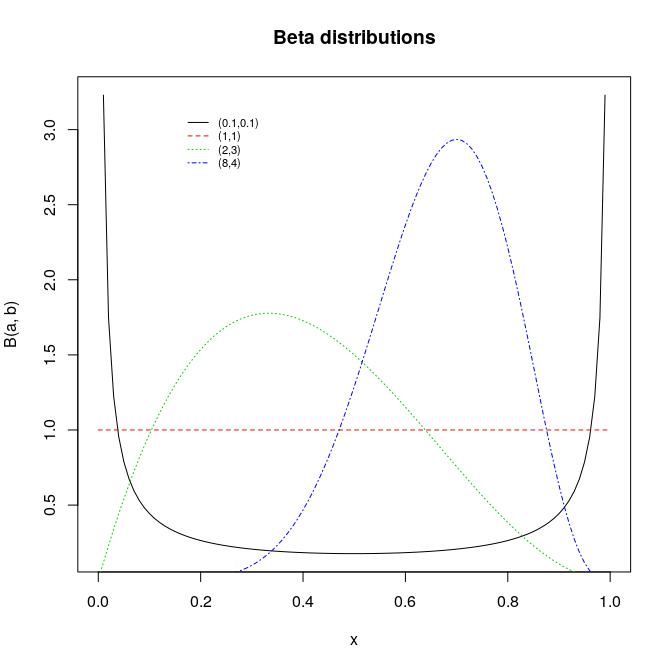
\includegraphics[scale=0.4]{c2f1}
\end{center}
\end{figure}

\item Let $X$ be a binomial random variable with probability mass function
\[
p(X = m|\mu) = \binom{N}{n}\mu^n (1 - \mu)^{N-n}.
\]
Let the parameter $\mu$ be described by a prior distribution
\begin{equation}\label{c2pe1}
\mathrm{Beta}(\mu|a, b) = \frac{\Gamma(a + b)}{\Gamma(a)\Gamma(b)}\mu^{a-1}(1 - \mu)^{b-1}.
\end{equation}
The observed data of $m + l$ realizations of $X$ has $x = 1$ $m$ times and $x = 0$ $l$ times.
Therefore, the likelihood function is
\[
p(\mathcal{D}|\mu) = \prod_{i=1}^{m}p(X=1|\mu)\prod_{j=1}^lp(X=0|\mu) = \mu^m(1 - \mu)^l.
\]
The posterior distribution of $\mu$ given the data $\mathcal{D}$ is
\[
p(\mu|D) \propto p(\mathcal{D}|\mu)\mathrm{Beta}(\mu|a, b) = \frac{\Gamma(a+b)}{\Gamma(a)\Gamma(b)}\mu^{m+a-1}(1-\mu)^{l+b-1}.
\]
The constant of proportionality is
\[
\frac{\Gamma(m+l+a+b)}{\Gamma(m+a)\Gamma(b+l)}
\]
so that
\[
p(\mu|\mathcal{D}) = \frac{\Gamma(m+l+a+b)}{\Gamma(m+a)\Gamma(b+l)}\mu^{m+a-1}(1-\mu)^{l+b-1}.
\]
The mean of $\mu$ conditioned on $\mathcal{D}$ is the posterior mean
\begin{equation}\label{c2pe2}
\mu_{post} = \frac{m+a}{m+a+l+b}.
\end{equation}

The log-likelihood function is
\[
\ln p(\mathcal{D}|\mu) = m\ln\mu + l\ln(1 - \mu)
\]
and its derivative is
\[
\frac{m}{\mu} - \frac{l}{1 - \mu}
\]
and its extremum is 
\begin{equation}\label{c2pe3}
\mu_{ML} = \frac{m}{m+l}.
\end{equation}
The mean of the prior distribution is that of equation \eqref{c2pe1}
\begin{equation}\label{c2pe4}
\mu_{prior} = \frac{a}{a+b}.
\end{equation}

Let us assume, for the moment that the maximum likelihood estimate is greater than the prior estimate.
That is,
\[
\mu_{ML} - \mu_{prior} > 0.
\]
This is possible if and only if 
\begin{equation}\label{c2pe5}
bm > al.
\end{equation}
If equation \eqref{c2pe5} is true then it is easy to verify that $\mu_{ML} > \mu_{post} > \mu_{prior}$. 
If \eqref{c2pe5} is not true then $\mu_{prior} \ge \mu_{post} \ge \mu_{ML}$.

\item Let $X$ and $Y$ be random variables with joint distribution $p(x, y)$. Then,
\[
\ev_x(X|Y) = \int xp(x|y)dx
\]
and 
\begin{eqnarray*}
\ev_y(\ev_x(X|Y)) &=& \int p(y)\ev_x(X|Y)dy \\
 &=& \iint xp(y)p(x|y)dxdy \\
 &=& \iint xp(x, y)dxdy \\
 &=& \ev(X).
\end{eqnarray*}

For sake of notational simplicity, let us denote $\ev_x(X|Y) = \phi(y)$. Then, 
\begin{equation}\label{c2pe6}
\var_y(\ev_x(X|Y)) = \var_y(\phi(y)) = \ev_y(\phi^2(y)) - (\ev_y\phi(y))^2
\end{equation}
Now, $\var_x(X|Y) = \ev_x(X^2|Y) - (\ev_x(X|Y))^2 = \ev_x(X^2|Y) - \phi^2(y)$ so that 
\[
\ev_y(\var_x(X|Y)) = \ev_y(\ev_x(X^2|Y)) - \ev_y(\phi^2(y))
\]
and hence
\[
\begin{split}
\var_y(\ev_x(X|Y)) + \ev_y(\var_x(X|Y)) =& \ev_y(\phi^2(y)) - (\ev_y\phi(y))^2 + \\
 & \ev_y(\ev_x(X^2|Y)) - \ev_y(\phi^2(y)) 
\end{split}
\]
and finally
\begin{equation}\label{c2pe7}
\var_y(\ev_x(X|Y)) + \ev_y(\var_x(X|Y)) = \ev_y(\ev_x(X^2|Y)) - (\ev_y\phi(y))^2 
\end{equation}
Now,
\begin{eqnarray*}
\ev_y(\ev_x(X^2|Y)) &=& \iint x^2 p(x|y)p(y)dxdy = \var(X) \\
\ev_y\phi(y) &=& \iint xp(x|y)p(y)dy = \ev(X)
\end{eqnarray*}
Using these in equation \eqref{c2pe7} we get the desired result.

\item We use the following result,
\begin{equation}\label{c2pe8}
\int_0^a x^{m-1}(a - x)^{n-1}dx = a^{m+n-1}B(m, n).
\end{equation}
To obtain it, we write the integral as
\[
a^{m+n-2}\int_0^a \left(\frac{x}{a}\right)^{m-1}\left(1 - \frac{x}{a}\right)^{n-1}ad\left(\frac{x}{a}\right).
\]
A transformation $x/a \mapsto y$ yields the result. The Dirichlet distribution is proportional
to 
\[
D = \prod_{k=1}^K\mu_k^{\alpha_k - 1}.
\]
subject to the constraint 
\begin{equation}\label{c2pe9}
\sum_{k=1}^K\mu_k = 1.
\end{equation}
Therefore, the distribution is proportional to
\[
D = \prod_{k=1}^{K-1}\mu_k^{\alpha_k - 1}(1 - \mu_1 - \cdots - \mu_{K-1})^{\alpha_K-1}
\]
The variables $\mu_k$ vary over $[0, 1]$. However, the constraint of equation \eqref{c2pe9} reduce the
region of integration from a hypercube to a $K-1$ simplex formed by the first quandrant and the plane whose 
equation is \eqref{c2pe9}. In order to find the normalization constant we must evaluate the integral
\begin{equation}\label{c2pe10}
I = \int_0^1\int_0^{1-\mu_1}\cdots\int_0^{1-\mu_1-\cdots-\mu_{K-2}}D(\mu_1, \ldots, \mu_{K-1})d\mu_1\cdots d\mu_{K-1}.
\end{equation}
The $\mu_{K-1}$ integral is
\begin{eqnarray*}
\int_0^{1-\mu_1-\cdots-\mu_{K-2}}\mu_{K-1}^{\alpha_K - 1}(1 - \mu_1 - \cdots - \mu_{K-1})^{\alpha_K-1}d\mu_{K-1} &=& \\
 (1-\mu_1-\cdots-\mu_{K-2})^{\alpha_K+\alpha_{K-1}-1}B(\alpha_K, \alpha_{K-1}) & &
\end{eqnarray*}
The integrals over the other variables are evaluated similarly so that
\[
I = B(\alpha_{K-1},\alpha_K)B(\alpha_{K-2},\alpha_{K}+\alpha_{K-1})\cdots B(\alpha_1,\alpha_{K}+\cdots+\alpha_2).
\]
Using the relation,
\[
B(m, n) = \frac{\Gamma(m)\Gamma(n)}{\Gamma(m+n)},
\]
we get
\begin{eqnarray*}
I &=& \frac{\Gamma(\alpha_{K-1})\Gamma(\alpha_K)}{\Gamma(\alpha_{K}+\alpha_{K-1})} \\
  & &  \frac{\Gamma(\alpha_{K-2})\Gamma(\alpha_K+\alpha_{K-1})}{\Gamma(\alpha_K+\alpha_{K-1}+\alpha_{K-2})}\cdots \\
  & &  \frac{\Gamma(\alpha_1)\Gamma(\alpha_K+\alpha_{K-1}+\cdots+\alpha_2)}{\Gamma(\alpha_K+\alpha_{K-1}+\cdots+\alpha_{1})}
\end{eqnarray*}
Cancelling common terms,
\[
I = \frac{\Gamma(\alpha_K)\Gamma(\alpha_{K-1})\cdots\Gamma(\alpha_1)}{\Gamma(\alpha_K+\alpha_{K-1}+\cdots+\alpha_1)}
\]
If we write $\alpha_0 = \alpha_1 + \cdots + \alpha_K$ then the normalization constant for the
Dirichlet distribution is
\[
\frac{\Gamma(\alpha_0)}{\Gamma(\alpha_1)\cdots\Gamma(\alpha_K)}.
\]

\item We start with the Dirichlet distribution
\[
\mathrm{Dir}(\mu|\alpha) = \frac{\Gamma(\alpha_0)}{\Gamma(\alpha_1)\cdots\Gamma(\alpha_K)}\prod_{k=1}^K\mu_k^{\alpha_k - 1},
\]
where $\mu, \alpha \in \sor^K$ and
\begin{eqnarray*}
\sum_{i=1}^K \mu_k &=& 1 \\
\sum_{i=1}^K \alpha_k &=& \alpha_0
\end{eqnarray*}
The mean of the distribution is
\begin{eqnarray*}
\ev(\mu_j) &=& \int\frac{\Gamma(\alpha_0)}{\Gamma(\alpha_1)\cdots\Gamma(\alpha_K)}\prod_{k=1}^K\mu_k^{\alpha_k + \delta_{jk} - 1}d\mu \\
 &=& \frac{\Gamma(\alpha_0)}{\Gamma(\alpha_1)\cdots\Gamma(\alpha_K)}\frac{\Gamma(\alpha_1)\cdots\Gamma(\alpha_j+1)\cdots\Gamma(\alpha_K)}{\Gamma(\alpha_0 + 1)} \\
 &=& \frac{\alpha_j}{\alpha_0}
\end{eqnarray*}
In order to find the variance, we need
\begin{eqnarray*}
\ev(\mu_j^2) &=& \int\frac{\Gamma(\alpha_0)}{\Gamma(\alpha_1)\cdots\Gamma(\alpha_K)}\prod_{k=1}^K\mu_k^{\alpha_k + 2\delta_{jk} - 1}d\mu \\
 &=& \frac{\Gamma(\alpha_0)}{\Gamma(\alpha_1)\cdots\Gamma(\alpha_K)}\frac{\Gamma(\alpha_1)\cdots\Gamma(\alpha_j+2)\cdots\Gamma(\alpha_K)}{\Gamma(\alpha_0 + 2)} \\
 &=& \frac{\alpha_j(\alpha_j+1)}{\alpha_0(\alpha_0+1)}
\end{eqnarray*}
Therefore,
\[
\var(\alpha_j) = \frac{\alpha_j(\alpha_j+1)}{\alpha_0(\alpha_0+1)} - \frac{\alpha_j^2}{\alpha_0^2} = \frac{\alpha_j(\alpha_0 - \alpha_j)}{\alpha_0^2(\alpha_0+1)}.
\]
Note that the definition of $\alpha_0$ guarantees us that the variance is non-negative. In order
to find the covariance, we need
\begin{eqnarray*}
\ev(\mu_i\mu_j) &=& \int\frac{\Gamma(\alpha_0)}{\Gamma(\alpha_1)\cdots\Gamma(\alpha_K)}\prod_{k=1}^K\mu_k^{\alpha_k + \delta_{ik} + \delta_{jk} - 1}d\mu \\
 &=& \frac{\Gamma(\alpha_0)}{\Gamma(\alpha_1)\cdots\Gamma(\alpha_K)}\frac{\Gamma(\alpha_1)\cdots\Gamma(\alpha_i+1)\cdots\Gamma(\alpha_j+1)\cdots\Gamma(\alpha_K)}{\Gamma(\alpha_0 + 2)} \\
 &=& \frac{\alpha_i\alpha_j}{\alpha_0(\alpha_0+1)}
\end{eqnarray*}
so that
\[
\cov(\mu_i\mu_j) = \frac{\alpha_i\alpha_j}{\alpha_0(\alpha_0+1)} - \frac{\alpha_i\alpha_j}{\alpha_0^2} = -\frac{\alpha_i\alpha_j}{\alpha_0^2(\alpha_0+1)}.
\]

\item Recall that the derivative of $a^x$ with respect to $x$ is $a^x\ln a$. Therefore,
\[
\frac{\partial}{\partial\alpha_j}\prod_{k=1}^K \mu_k^{\alpha_k-1} = \ln\mu_j\prod_{k=1}^K\mu_k^{\alpha_k-1}.
\]
Now,
\begin{eqnarray*}
\ev(\ln\mu_j) &=& \frac{\Gamma(\alpha_0)}{\Gamma(\alpha_1)\cdots\Gamma(\alpha_K)}\int\ln\mu_j\prod_{k=1}^K\mu_k^{\alpha_k-1}d\mu \\
 &=& \frac{\Gamma(\alpha_0)}{\Gamma(\alpha_1)\cdots\Gamma(\alpha_K)}\int\frac{\partial}{\partial\alpha_j}\prod_{k=1}^K\mu_k^{\alpha_k-1}d\mu \\
 &=& \frac{\Gamma(\alpha_0)}{\Gamma(\alpha_1)\cdots\Gamma(\alpha_K)}\frac{\partial}{\partial\alpha_j}\int\prod_{k=1}^K\mu_k^{\alpha_k-1}d\mu \\
 &=& \frac{\Gamma(\alpha_0)}{\Gamma(\alpha_1)\cdots\Gamma(\alpha_K)}\frac{\partial}{\partial\alpha_j}\frac{\Gamma(\alpha_1)\cdots\Gamma(\alpha_K)}{\Gamma(\alpha_0)} \\
 &=& \frac{\Gamma(\alpha_0)}{\Gamma(\alpha_j)}\frac{\partial}{\partial\alpha_j}\frac{\Gamma(\alpha_j)}{\Gamma(\alpha_0)} \\
 &=& \frac{1}{\Gamma(\alpha_j)}\frac{\partial}{\partial\alpha_j}\Gamma(\alpha_j) - \frac{1}{\Gamma(\alpha_0)}\frac{\partial}{\partial\alpha_j}\Gamma(\alpha_0) \\
 &=& \frac{\partial}{\partial\alpha_j}\ln\Gamma(\alpha_j) - \frac{\partial}{\partial\alpha_j}\ln\Gamma(\alpha_0) \\
 &=& \psi(\alpha_j) - \psi(\alpha_0),
\end{eqnarray*}
where 
\[
\psi(\alpha) = \frac{d}{d\alpha}\ln\Gamma(\alpha)
\]
is the digamma function.

\item The uniform distribution is defined by
\[
\mathrm{Unif}(x|a, b) = \frac{1}{b - a}, x \in [a, b].
\]
It is easy to confirm that it is normalized, for
\[
\int_a^b \mathrm{Unif}(x|a, b)dx = \frac{1}{b-a}\int_a^b dx = 1.
\]
The mean value of $x$ is
\[
\ev(x) = \int_a^b x\mathrm{Unif}(x|a, b)dx = \int_a^b \frac{x}{b-a}dx = \frac{1}{2(b-a)}(b^2 - a^2) = \frac{a+b}{2}.
\]
The mean value of $x^2$ is
\[
\ev(x^2) = \int_a^b\frac{x^2}{b-a}dx = \frac{1}{3(b-a)}(b^3-a^3) = \frac{a^2 + ab + b^2}{3}
\]
so that 
\[
\var(x) = \frac{a^2 + ab + b^2}{3} - \frac{(a+b)^2}{4} = \frac{(b - a)^2}{12}.
\]

\item Given that
\begin{eqnarray*}
p(x) &=& \mathcal{N}(x | \mu, \Sigma) \\
q(x) &=& \mathcal{N}(x | m, L),
\end{eqnarray*}
where $x, \mu, m \in \sor^n$ and $\Sigma, L$ are covariance matrices.
\[
\ln\left(\frac{q(x)}{p(x)}\right) = \frac{1}{2}\ln\frac{\det L}{\det\Sigma} - \frac{(x - m)^TL^{-1}(x - m)}{2} + \frac{(x - \mu)^T\Sigma^{-1}(x - \mu)}{2}.
\]
The Kullback-Leibler divergence between $p$ and $q$ is the sum of three integrals,
\begin{eqnarray*}
I_1 &=& -\frac{1}{2}\ln\left|\frac{\det L}{\det\Sigma}\right|\int_{\sor^n}p(x)dx \\
I_2 &=& \frac{1}{2}\int_{\sor^n}(x-m)^TL^{-1}(x-m)p(x)dx \\
I_3 &=& -\frac{1}{2}\int_{\sor^n}(x-\mu)^T\Sigma^{-1}(x-\mu)p(x)dx.
\end{eqnarray*}
It is easy to evaluate $I_1$ using normalization property of $p$.
\begin{equation}\label{c2pe11}
I_1 = -\frac{1}{2}\ln\left|\frac{\det L}{\det\Sigma}\right|.
\end{equation}
Using the definitions of expectations, we conclude that
\[
I_2 = \ev[(x - m)^TL^{-1}(x-m)].
\]
Using formula (380) of the matrix cookbook \cite{petersen2012matrix} we get
\begin{equation}\label{c2pe12}
I_2 = (m - \mu)^TL^{-1}(m - \mu) + \tr(L^{-1}\Sigma).
\end{equation}
In eaxctly the same manner, we conclude that
\begin{equation}\label{c2pe13}
I_3 = 0 + \tr(\Sigma^{-1}\Sigma) = n.
\end{equation}
Therefore,
\[
\kl(p||q) = -\frac{1}{2}\left(\ln\left|\frac{\det L}{\det\Sigma}\right| - (m - \mu)^T L^{-1}(m - \mu) + \tr(L^{-1}\Sigma) + d\right).
\]

\item Let $x, \mu \in \sor^n$ and $\Sigma$ be an $n \times n$ covariance matrix. The entropy of a 
distribution is given by
\[
H = -\int p(x)\ln p(x)dx.
\]
We want to maximize $H$ subject to the constraints
\begin{eqnarray}
\int p(x)dx &=& 1 \label{c2pe14} \\
\int xp(x)dx &=& \mu \label{c2pe15} \\
\int (x - \mu)(x - \mu)^Tp(x)dx &=& \Sigma \label{c2pe16} .
\end{eqnarray}
If $\lambda_1, \ell, \lambda_3$ are the Lagrange multipliers for each of these constraints then
we seek to maximize the functional
\begin{eqnarray*}
L[x] &=& H - \lambda_1\left(\int p(x)dx - 1\right) - \ell^T\left(\int xp(x)dx - \mu\right) - \\
 & & \Lambda\left(\int(x-\mu)^T(x-\mu)p(x)dx - \Sigma\right),
\end{eqnarray*}
where $\lambda_1 \in \sor, \ell \in \sor^n$ and $\Lambda$ is an $n \times n$ non-singular 
symmetric matrix. Each term on the right hand side is a number. Therefore, it is equal to the
trace of itself. We use this fact on the third term to get
\begin{eqnarray*}
L[x] &=& H - \lambda_1\left(\int p(x)dx - 1\right) - \ell^T\left(\int xp(x)dx - \mu\right) - \\
 & & \tr\left\{\Lambda\left(\int(x-\mu)^T(x-\mu)p(x)dx - \Sigma\right)\right\},
\end{eqnarray*}
 We now take the functional derivative of the above equation with respect to $p$,
\[
\frac{\delta L}{\delta p} = -1 - \ln p(x) - \lambda_1 - \ell^T x - \tr(\Lambda (x - \mu)^T(x - \mu)).
\]
As $\tr(AB) = \tr(BA)$, we can write the last expression on the right hand side as
\[
\frac{\delta L}{\delta p} = -1 - \ln p(x) - \lambda_1 - \ell^T x - \tr((x - \mu)^T\Lambda(x - \mu)).
\]
At an extremum of $L$, the functional derivative vanishes so that $\ln p(x) = -1 - \lambda_1 - \ell x
- (x - \mu)^T\Lambda(x - \mu)$ or
\begin{equation}\label{c2pe17}
p(x) = \exp\left(-1 - \lambda_1 - \ell^T x - (x - \mu)^T\Lambda(x - \mu)\right).
\end{equation}
We now write 
\begin{eqnarray*}
\ell^T x &=& \ell^T \Lambda^{-1} \Lambda x + \mu^T\ell - \mu^T\ell \\
 &=&  \ell^T \Lambda^{-1} \Lambda x + \mu^T\ell - \ell^T\mu \\
 &=& \ell^T\Lambda^{-1}\Lambda(x - \mu) + \mu^T\ell.
\end{eqnarray*}
We used the fact that $\mu^T\ell = (\mu, \ell) = (\ell, \mu) = \ell^T\mu$ as all
the vectors are real. Since $\Lambda$ is symmetric, so is its inverse and hence $\Lambda^{-1}
= (\Lambda^{-1})^T$. Therefore,
\begin{eqnarray*}
\ell^T x &=& (\ell\Lambda^{-1})^T\Lambda(x - \mu) + \mu^T\ell \\
 &=& \frac{(\ell\Lambda^{-1})^T\lambda_x(x - \mu)}{2} + \frac{(x - \mu)^T\Lambda^T\Lambda^{-1}\ell}{2} + \mu^T\ell
\end{eqnarray*}
and hence
\begin{eqnarray*}
\ell^Tx + (x-\mu)^T\Lambda(x-\mu) &=& \left(x-\mu+\frac{\Lambda^{-1}\ell}{2}\right)^T\Lambda\left(x-\mu+\frac{\Lambda^{-1}\ell}{2}\right) \\
 & & \mu^T\ell - \frac{\ell^T\Lambda^{-1}\ell}{4}
\end{eqnarray*}
The density $p$ can now be written as
\[
p(x)=\exp\left[-1-\lambda_1 - \left(x-\mu+\frac{\Lambda^{-1}\ell}{2}\right)^T\Lambda\left(x-\mu+\frac{\Lambda^{-1}\ell}{2}\right)-\mu^T\ell+\frac{\ell^T\Lambda^{-1}\ell}{4}\right]
\]
Introduce a variable 
\[
y = x - \mu + \frac{\Lambda^{-1}\ell}{2}
\]
so that the density becomes
\[
p(y) = \exp\left[-1-\lambda_1-y^T\Lambda y - \mu^T\ell - \frac{\ell^T\Lambda^{-1}\ell}{4}\right].
\]
We use this form in the second constraint to get
\[
\int\left(y + \mu + \frac{\Lambda^{-1}\ell}{2}\right)p(y)dy = \mu.
\]
The integral of $yp(y)$ vanishes because it is an odd function. The rest of the term evaluates to
\[
\mu + \frac{\Lambda^{-1}\ell}{2} = \mu
\]
or $\Lambda^{-1}\ell = 0$. As $\Lambda$ is a non-singular symmetric matrix, this means that $\ell = 0$.
The form of the density now simplifies to
\[
p(y) = \exp\left(-1 - \lambda_1 - y^T\Lambda y\right),
\]
where $y$ now is just $x - \mu$. We now use this form in the third constraint. We define 
$y = x - \mu$ so that
\begin{equation}\label{c2pe18}
\int yy^Te^{-1 - \lambda_1 - y^T\Lambda y}dy = \Sigma \Rightarrow e^{-1-\lambda_1} \int yy^T e^{-y^T\Lambda y}dy = \Sigma.
\end{equation}
In order to evaluate this integral we use the eigenvalues of $\Lambda$. Let $\Lambda u_i = \alpha_i u_i$,
where $u_i$ is an eigenvector corresponding to the eigenvalue $\alpha_i$. We can then write 
\[
y = \sum_{i=1}^n \beta_i u_i,
\]
where $\beta_i = u_i^T y = (u_i, y)$. The $n$ numbers $\beta_i$ form a vector $\beta$ and we can write
\begin{equation}\label{c2pe19}
\beta = Uy,
\end{equation}
where the matrix $U = [u_1 \ldots u_n]$ has the eigenvectors of $\Lambda$ as its columns. From \eqref{c2pe19}
we readily get 
\begin{equation}\label{c2pe20}
d\beta = \abs{\det U}dy.
\end{equation}
If we choose the eigenvectors to be orthonormal then $\abs{\det U} = 1$ and 
\begin{equation}\label{c2pe21}
d\beta = dy.
\end{equation}
Therefore,
\[
y^T\Lambda y = \sum_{i,j=1}^n \beta_i u_i^T \Lambda \beta_j u_j = \sum_{i,j=1}^n \beta_i\beta_j\alpha_j u_i^T u_j,
\]
where $\alpha_j$ is the eigenvalue of $u_j$. As the eigenvectors $\{u_i\}$ can always be 
assumed to be orthonormal, $(u_i, u_j) = \delta_{ij}$ and hence
\[
y^T\Lambda y = \sum_{i=1}^n \beta_j^2\alpha_i
\]
Recall that $\Lambda$ is a constant matrix. Therefore, its eigenvectors are also constant and hence
\[
y = \sum_{i=1}^n\beta_i u_i \Rightarrow dy = \sum_{i=1}^n u_i d\beta_i
\]
Equation \eqref{c2pe18} now becomes
\begin{equation}\label{c2pe22}
e^{-1+\lambda_1}\sum_{i,j=1}^nu_iu_j^T\int \exp\left(-\sum_{k=1}^n\beta_k^2\alpha_k\right)\beta_i\beta_j d\beta = \Sigma.
\end{equation}
The integral in the above equation is zero if $i \ne j$. When $i = j$, it becomes
\[
I = \int e^{-\beta_1^2\alpha_1}d\beta_1 \cdots \int \beta_i^2e^{-\beta_i^2\alpha_i}d\beta_i \cdots \int e^{-\beta_n^2\alpha_n}d\beta_n = \frac{\pi^{n/2}}{\sqrt{\alpha_1 \cdots \alpha_n}}\frac{1}{2\alpha_i}.
\]
Equation \eqref{c2pe22} then becomes
\[
e^{-1-\lambda_1}\sqrt{\frac{\pi^n}{\alpha_1\cdots\alpha_n}}\sum_{i=1}^n \frac{1}{2\alpha_i}u_iu_i^T = \Sigma.
\]
Since $\Lambda u_i = \alpha_i u_i$, the expression sum in the above equation is really $\Lambda^{-1}/2$.
(Refer to equations (2.48) and (2.49) of the book.). Therefore,
\[
e^{-1 - \lambda_1}\sqrt{\frac{\pi^n}{\alpha_1\cdots\alpha_n}}\frac{1}{2}\Lambda^{-1} = \Sigma.
\]
The determinant of a matrix is a product of its eigen-values. Therefore,
\[
\frac{e^{-1 - \lambda_1}}{2}\frac{\pi^{n/2}}{\sqrt{\det\Lambda}}\Lambda^{-1} = \Sigma.
\]
We now choose $\Lambda^{-1} = 2\Sigma$ so that
\begin{equation}\label{cpe23}
\Lambda = \frac{1}{2}\Sigma^{-1}.
\end{equation}
and $\lambda_1$ such that 
\[
e^{-1 - \lambda_1}\frac{\pi^{n/2}}{\sqrt{\det\Lambda}} = 1 \Rightarrow e^{-1-\lambda_1} = \frac{\sqrt{\det\Lambda}}{\pi^{n/2}}.
\]
From equation \eqref{cpe23}, 
\[
\det\Lambda = \frac{1}{2^n}\det\Sigma^{-1} = \frac{1}{2^n}\frac{1}{\det\Sigma}
\]
so that
\begin{equation}\label{cpe24}
e^{-1 - \lambda_1} = \frac{1}{(2\pi)^{n/2}}\frac{1}{\sqrt{\det\Sigma}}.
\end{equation}
Equations \eqref{cpe23}, \eqref{cpe24} and the fact that $\ell = 0$ make the $p$ a multi-variate
gaussian distribution.

\item The entropy of a distribution $p$ is
\[
H = -\int p(x)\ln p(x)dx.
\]
If $p$ is a multivariate gaussian distribution,
\[
p(x) = \frac{1}{(2\pi)^{n/2}}\frac{1}{\sqrt{\det\Sigma}}\exp\left(-\frac{(x - \mu)^T\Sigma^{-1}(x - \mu)}{2}\right)
\]
so that
\[
\ln p = -\frac{n}{2}\ln(2\pi) - \frac{1}{2}\ln\det\Sigma - \frac{(x - \mu)^T\Sigma^{-1}(x - \mu)}{2}
\]
Therefore,
\[
H = \frac{n}{2}\ln(2\pi) + \frac{1}{2}\ln\det\Sigma + \frac{1}{2}\int(x - \mu)^T\Sigma^{-1}(x - \mu)p(x)dx.
\]
The integral $I$ is best evaluated using the property of expectations. Clearly, $I = \ev((x-\mu)^T\Sigma^{-1}(x-\mu))$.
As $(x-\mu)^T\Sigma^{-1}(x-\mu)$ is a number, we can as well write
\begin{eqnarray*}
I &=& \ev(\tr((x - \mu)^T\Sigma^{-1}(x - \mu))) \\
  &=& \ev(\tr(\Sigma^{-1}(x - \mu)^T(x - \mu))) \\
  &=& \ev(\tr(\Sigma^{-1})\tr((x - \mu)^T(x - \mu))) \\
  &=& \tr(\Sigma^{-1})\ev(\tr((x - \mu)^T(x - \mu))) \\
  &=& \tr(\Sigma^{-1})\tr(\ev(x - \mu)^T(x - \mu)) \\
  &=& \tr(\Sigma^{-1})\tr(\Sigma) \\
  &=& \tr(\Sigma^{-1}\Sigma) = n
\end{eqnarray*}
The entropy is thus,
\[
H = \frac{1}{2}\ln\det\Sigma + \frac{n}{2}\left(1 + \ln(2\pi)\right).
\]

\item Given that the random variable $X$ is a sum of two gaussian random variables $X_1$ and $X_2$.
The probability that $X$ takes a value between $x$ and $x + dx$ is $p(x)dx$. This is equal to the
probability that $X_2$ takes a value between $x_2$ and $dx_2$ and $X_1$ takes a value between $x - x_2$
and $d(x - x_2)$. Thus,
\[
p(x) = \int_\sor p(x - x_2)p(x_2)dx_2.
\]
The integral on the right is called a convolution of $p$ with itself. Given that
\[
p(x_2) = \sqrt{\frac{\tau_2}{2\pi}}e^{-(x_2 - \mu_2)^2\tau_2}
\]
and
\[
p(x - x_2) = \sqrt{\frac{\tau_1}{2\pi}}e^{-(x - x_2 - \mu_1)^2\tau_1}
\]
so that
\[
p(x) = \frac{\sqrt{\tau_1\tau_2}}{2\pi}\int_\sor e^{-[(x - x_2 - \mu_1)^2\tau_1 + (x_2 - \mu_2)^2\tau_2]}dx_2
\]
In order to proceed, we must simplify the argument of the exponent. It is
\begin{eqnarray*}
&=& (x - \mu_1)^2\tau_1 - 2(x - \mu_1)\tau_1x_2 + x_2^2\tau_1 + x_2^2\tau_2 - 2x_2\mu_2\tau_2 + \mu_2^2\tau_2 \\
&=& (\tau_1 + \tau_2)x_2^2 -2[(x - \mu_1)\tau_1 + \mu_2\tau_2]x_2 + (x - \mu_1)^2\tau_1 + \mu_2^2\tau_2 \\
&=& (\tau_1 + \tau_2)x_2^2 -2[(x - \mu_1)\tau_1 + \mu_2\tau_2]x_2 + \frac{[(x - \mu_1)\tau_1 + \mu_2\tau_2]^2}{\tau_1 + \tau_2} - \\
& & \frac{[(x - \mu_1)\tau_1 + \mu_2\tau_2]^2}{\tau_1 + \tau_2} - (x - \mu_1)^2\tau_1 + \mu_2^2\tau_2 \\
&=& \left(\sqrt{\tau_1 + \tau_2}x_2 - \frac{[(x - \mu_1)\tau_1 + \mu_2\tau_2]}{\sqrt{\tau_1 + \tau_2}}\right)^2 - \\
& & \frac{[(x - \mu_1)\tau_1 + \mu_2\tau_2]^2}{\tau_1 + \tau_2} - (x - \mu_1)^2\tau_1 + \mu_2^2\tau_2 \\
\end{eqnarray*}
The expression for density is
\[
\begin{split}
p(x) = & \frac{\sqrt{\tau_1\tau_2}}{2\pi}\exp\left(-\frac{[(x - \mu_1)\tau_1 + \mu_2\tau_2]^2}{\tau_1 + \tau_2} + (x - \mu_1)^2\tau_1 + \mu_2^2\tau_2\right) \\
 & \int_\sor\exp\left(-\left(\sqrt{\tau_1 + \tau_2}x_2 - \frac{[(x - \mu_1)\tau_1 + \mu_2\tau_2]}{\sqrt{\tau_1 + \tau_2}}\right)^2\right)dx_2
\end{split}
\]
In order to evaluate the integral, introduce the variable
\[
y = \sqrt{\tau_1 + \tau_2}x_2 - \frac{[(x - \mu_1)\tau_1 + \mu_2\tau_2]}{\sqrt{\tau_1 + \tau_2}}
\]
so that
\[
dx_2 = \frac{dy}{\sqrt{\tau_1 + \tau_2}}
\]
and hence
\[
\begin{split}
p(x) = & \frac{\sqrt{\tau_1\tau_2}}{2\pi}\exp\left(-\frac{[(x - \mu_1)\tau_1 + \mu_2\tau_2]^2}{\tau_1 + \tau_2} + (x - \mu_1)^2\tau_1 + \mu_2^2\tau_2\right) \\
 & \frac{1}{\sqrt{\tau_1+\tau_2}}\int_\sor e^{-y^2}dy.
\end{split}
\]
Simplifying further,
\[
p(x) = \frac{1}{2\sqrt{\pi}}\sqrt{\frac{\tau_1\tau_2}{\tau_1 + \tau_2}}\exp\left(-\frac{[(x - \mu_1)\tau_1 + \mu_2\tau_2]^2}{\tau_1 + \tau_2} + (x - \mu_1)^2\tau_1 + \mu_2^2\tau_2\right) 
\]
Let
\begin{eqnarray*}
\frac{1}{\tau} &=& \frac{1}{\tau_1} + \frac{1}{\tau_2} \\
\mu &=& \mu_1 + \mu_2
\end{eqnarray*}
then
\[
p(x) = \frac{1}{2}\sqrt{\frac{\tau}{\pi}}\exp\left(-(x - \mu)^2\tau\right).
\]
This is a gaussian with mean $\mu$ and precision $\tau$. Therefore, its entropy is
\[
H(p) = \frac{1}{2}\left(1 + \ln\left(\frac{2\pi}{\tau}\right)\right).
\]

\item Consider the multivariate gaussian
\[
\mathcal{N}(x|\mu,\Sigma) = \frac{1}{(2\pi)^{n/2}}\frac{1}{\sqrt{\det\Sigma}}\exp\left(-\frac{(x - \mu)^T\Sigma^{-1}(\mu - \tau)}{2}\right).
\]
We can write any matrix as a sum of a symmetric and an anti-symmetric matrix. For,
\[
\Sigma^{-1} = \frac{\Sigma^{-1} + (\Sigma^{-1})^T}{2} + \frac{\Sigma^{-1} - (\Sigma^{-1})^T}{2}.
\]
Now the argument of the exponent can be written as
\begin{eqnarray*}
 &=& (x - \mu)^T(\Sigma^{-1} - (\Sigma^{-1})^T)(x - \mu) \\
 &=& (x - \mu)^T\Sigma^{-1}(x - \mu) - (x - \mu)^T(\Sigma^{-1})^T(x - \mu) \\
 &=& \sum_{i,j=1}^n(x - \mu)_i\Sigma^{-1}_{ij}(x - \mu)_j - \sum_{i,j=1}^n((x - \mu)_i((\Sigma^{-1}_{ji}(x - \mu)_j \\
 &=& \sum_{i,j=1}^n(x - \mu)_i\Sigma^{-1}_{ij}(x - \mu)_j - \sum_{i,j=1}^n((x - \mu)_j((\Sigma^{-1}_{ji}(x - \mu)_i \\
 &=& 0.
\end{eqnarray*}
Likewise, it is easy to show that
\[
(x - \mu)^T(\Sigma^{-1} + (\Sigma^{-1})^T)(x - \mu) = (x - \mu)^T\Sigma^{-1}(x - \mu)
\]
so that not only the symmetric part survives, it is also identical to the original term.

\item Let $\Sigma u = \lambda u$. Take the hermitian adjoint of this equation, $\bar{u}^T\Sigma^\ast
= \bar{u}^T\bar{\lambda}$. Since $\Sigma$ is real and symmetric, $\Sigma^\ast = \Sigma$ and hence
$\bar{u}^T\Sigma = \bar{u}^T\bar{\lambda}$. From the original equation, we have $\bar{u}^T\Sigma u = 
\lambda \bar{u}^T u$. From the latter equation we get $\bar{u}^T\Sigma u = \bar{\lambda}\bar{u}^T u$.
The left hand sides of these equations are identical. Therefore, $\bar{\lambda} = \lambda$.

Let $\Sigma u_1 = \lambda_1 u_1$ and $\Sigma u_2 = \lambda u_2$. Then,
\begin{eqnarray*}
u_2^T\Sigma u_1 &=& \lambda_1 u_2^T u_1 \\
u_1^T\Sigma u_2 &=& \lambda_2 u_1^T u_1.
\end{eqnarray*}
Take the transpose of the second equation. Since $\Sigma$ is symmetric
\[
u_2^T\Sigma u_1 = \lambda_2 u_2^T u_1.
\]
Subtract this equation from the first one to get $0 = (\lambda_1 - \lambda_2)(u_2, u_1)$. Since the 
two eigenvalues are distinct, $(u_2, u_1) = 0$. This conclusion is valid even if one of the eigenvalues
is zero.

\item Let $u_1, \ldots, u_n$ be the eigenvectors of $\Sigma$ and $\lambda_1, \ldots, \lambda_n$ be
the corresponding eigenvalues. Form the $n \times n$ matrix $U = [u_1 \ldots u_n]$. We also assume
that $u_i$'s are orthonormal. Let $M = U\Lambda U^T$, where $\Lambda = \diag(\lambda_1, \ldots,
\lambda_n)$. Then, $U^TM U = U^TU \Lambda U^TU = \Lambda$.

Since $\Sigma u_i = \lambda_i u_i$, we also have $U^T\Sigma U = \Lambda$. Therefore, $U^T M U = U^T \Lambda U
\Rightarrow UU^T M UU^T = UU^T \Lambda UU^T \Rightarrow M = U$.

Now consider 
\[
\sum_{i=1}^n \lambda_i u_i u_i^T\sum_{j=1}^n\frac{1}{\lambda_j}u_j u_j^T =
\sum_{i,j=1}^n\frac{\lambda_i}{\lambda_j}u_i u_i^T u_j u_j^T =
\sum_{i,j=1}^n \frac{\lambda_i}{\lambda_j}u_i\delta_{ij}u_j^T = \sum_{i=1}^n u_iu_i^T = I.
\]
The last equality follows from the completeness property of vector spaces. Therefore, the
matrix
\[
\sum_{i=1}^n\frac{1}{\lambda_i}u_i u_i^T
\]
is the inverse of $\Sigma$.

\item Let $u_1, \dots, u_n$ be eigenvectors of $\Sigma$ with eigenvalues $\lambda_1, \ldots,
\lambda_n$. The eigenvectors also form the basis of $\sor^n$ so that any vector $a$ can be
expressed as
\[
a = \sum_{i=1}^n \mu_i u_i.
\]
Therefore, 
\[
a^T\Sigma a = \sum_{i,j=1}^n \mu_i \mu_j u_i^T \Sigma u_j = \sum_{i,j=1}^n \mu_i\mu_j\lambda_j u_i^T u_j = \sum_{i,j=1}^n\mu_i\mu_j\lambda_j\delta_{ij},
\]
or
\[
a^T\Sigma a = \sum_{i=1}^n \mu_i^1\lambda_i.
\]
From this equation it is clear that if $\lambda_i \ge 0$ for all $i$ then $a^T\Sigma a \ge 0$.

Now assume that $a^T\Sigma a \ge 0$ for all $a$. Therefore, in particular, $u_i^T\Sigma u_i \ge 0
\Rightarrow \lambda_i u_i^T u_i \ge 0$. Since $(u_i, u_i) > 0$, this just means $\lambda_i \ge 0$.

\item There are $D$ diagonal elements and $0 + 1 + \cdots + (D - 1)$ lower diagonal elements. The
latter sum is $(D - 1)D/2$. Therefore, the total number of independent elements is
\[
D + \frac{1}{2}D(D - 1) = \frac{1}{2}D(D + 1).
\]

\item Let $A$ be a symmetric matrix. Therefore, $A = A^T$. We know that $A^{-1}A = I$ so that
$A^T(A^{-1})^T = I \Rightarrow A (A^{-1})^T = I$, which means that $(A^{-1})^T$ is also an inverse
of $A$. But the inverse of a matrix is unique. Therefore, $A^{-1} = (A^{-1})^T$.
\end{enumerate}

